%================================================================
\section{Results and Discussion}\label{sec:Results}
%================================================================

The procedures for producing the following results are contained in Jupyter Notebooks found here:
\begin{center}
    \url{https://github.com/nicolossus/FYS-STK4155-Project2/tree/master/notebooks}
\end{center}

The associated source code can similarly be found here: 
\begin{center}
    \url{https://github.com/nicolossus/FYS-STK4155-Project2/tree/master/src}
\end{center}

%----------------------------------------------------------------
\subsection{Producing Data for 1D Ising Model}\label{sec:results datagen}
%----------------------------------------------------------------

Discuss counting in the all-to-all Ising model

%----------------------------------------------------------------
\subsection{Learning the Ising Hamiltonian with Linear Regression}\label{sec:results linreg}
%----------------------------------------------------------------

\autoref{fig:j_ols} shows the coupling matrix obtained by performing OLS regression.

\begin{figure}[H]
\begin{center}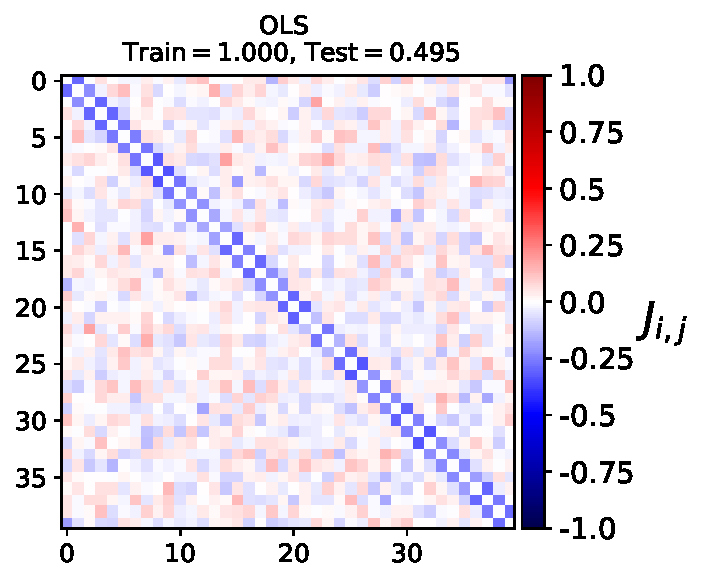
\includegraphics[scale=0.6]{latex/figures/ising_J_ols.pdf}
\end{center}
\caption{figure text}
\label{fig:j_ols}
\end{figure}

\autoref{fig:j_lmbda} shows the coupling matrices obtained by performing Ridge and Lasso regression with different regularization parameter, $\lambda$, values.

\begin{figure}[H]
\captionsetup[subfigure]{labelformat=empty}
\centering
\subfloat[]{{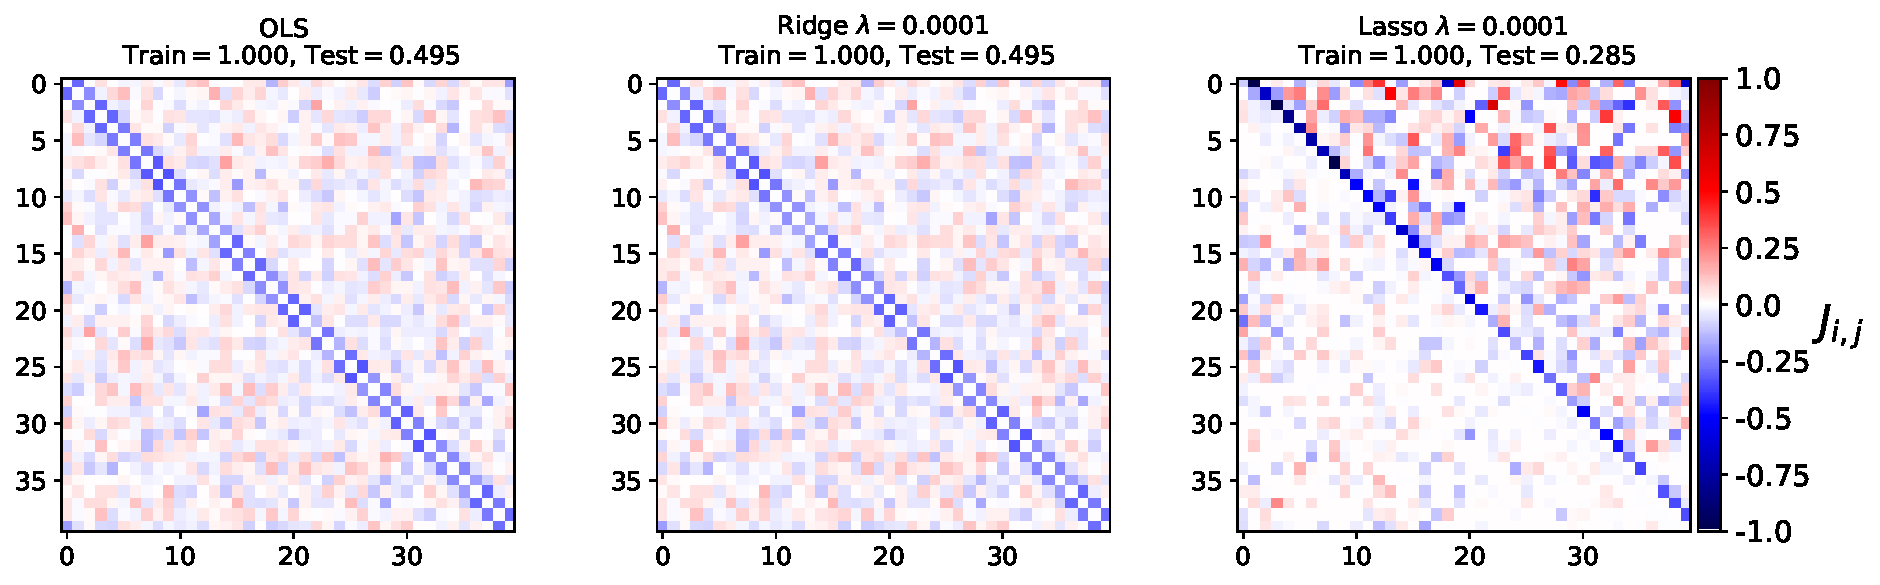
\includegraphics[scale=0.35]{latex/figures/ising_J_lmbda_0_0001.pdf}}}
\qquad
\subfloat[]{{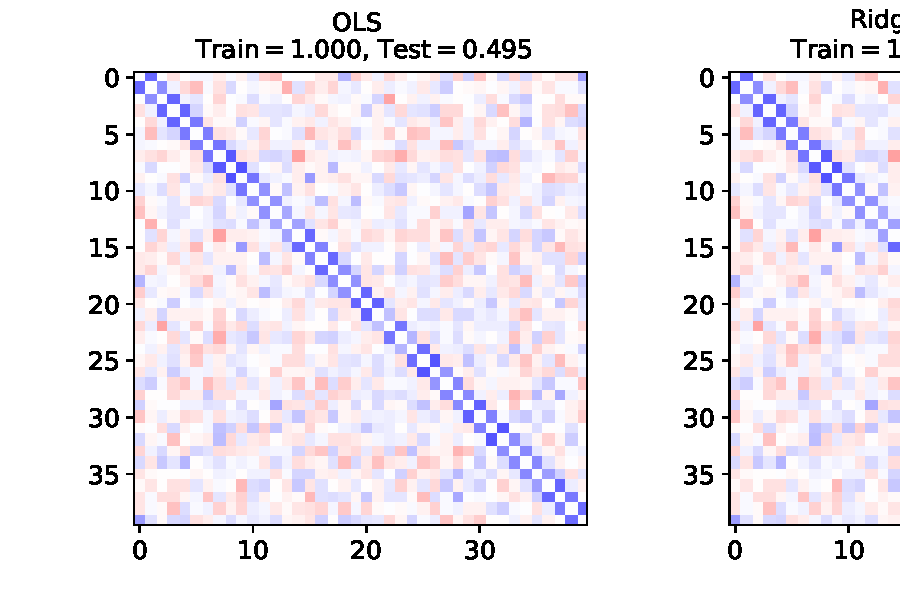
\includegraphics[scale=0.35]{latex/figures/ising_J_lmbda_0_001.pdf}}}
\qquad
\subfloat[]{{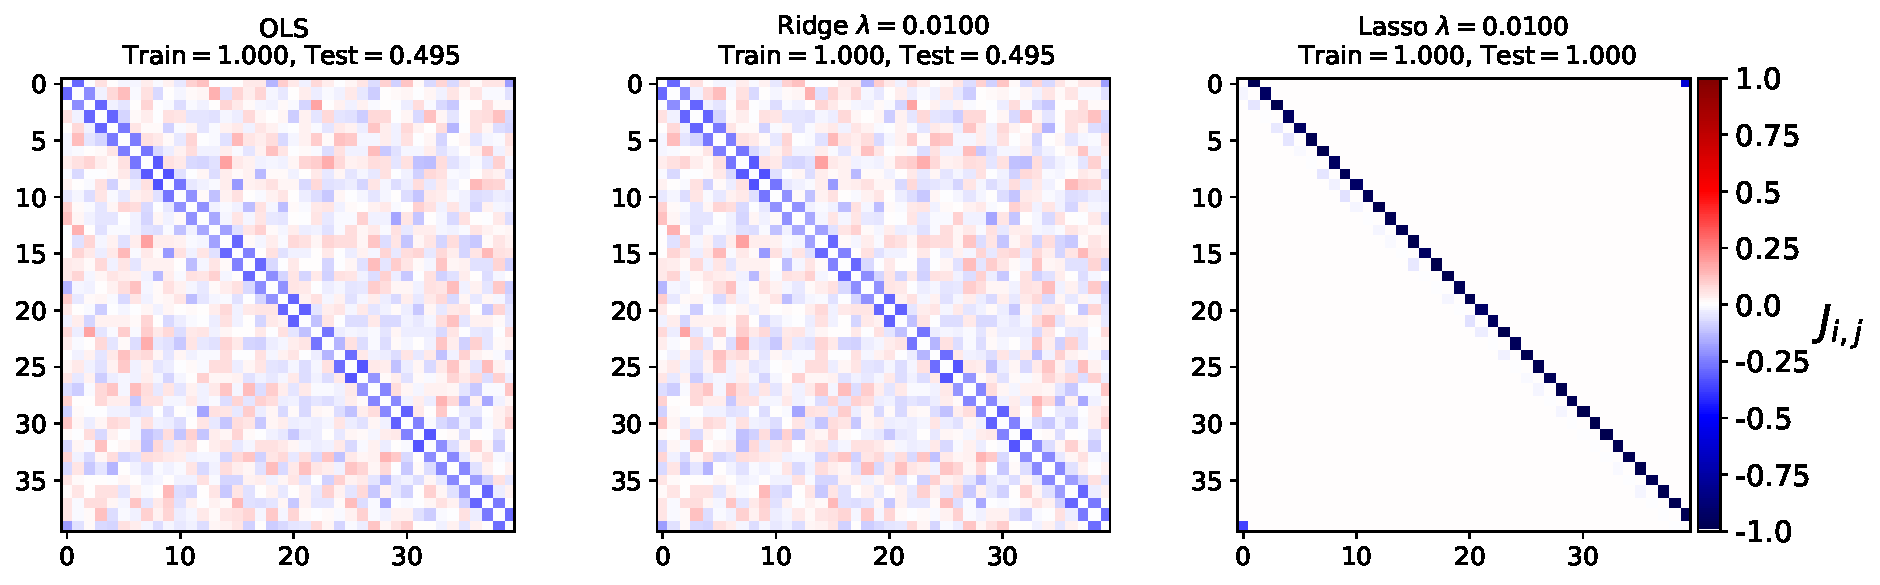
\includegraphics[scale=0.35]{latex/figures/ising_J_lmbda_0_01.pdf}}}
\qquad
\subfloat[]{{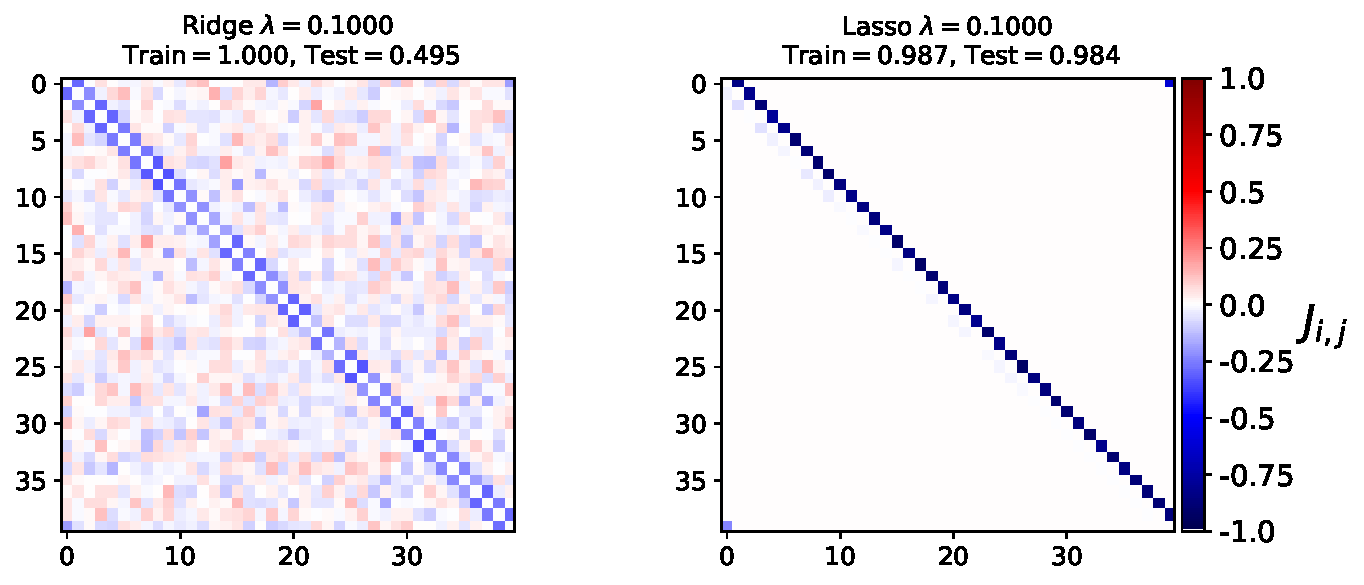
\includegraphics[scale=0.35]{latex/figures/ising_J_lmbda_0_1.pdf}}}
\qquad
\subfloat[]{{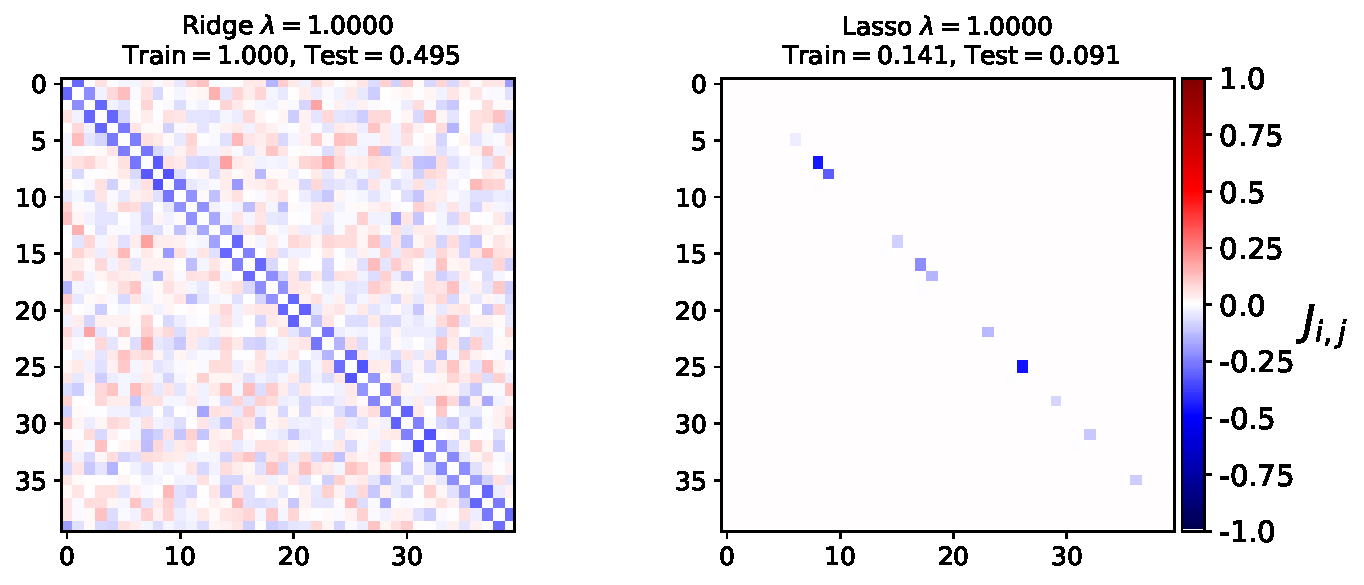
\includegraphics[scale=0.35]{latex/figures/ising_J_lmbda_1_0.pdf}}}
\qquad
\subfloat[]{{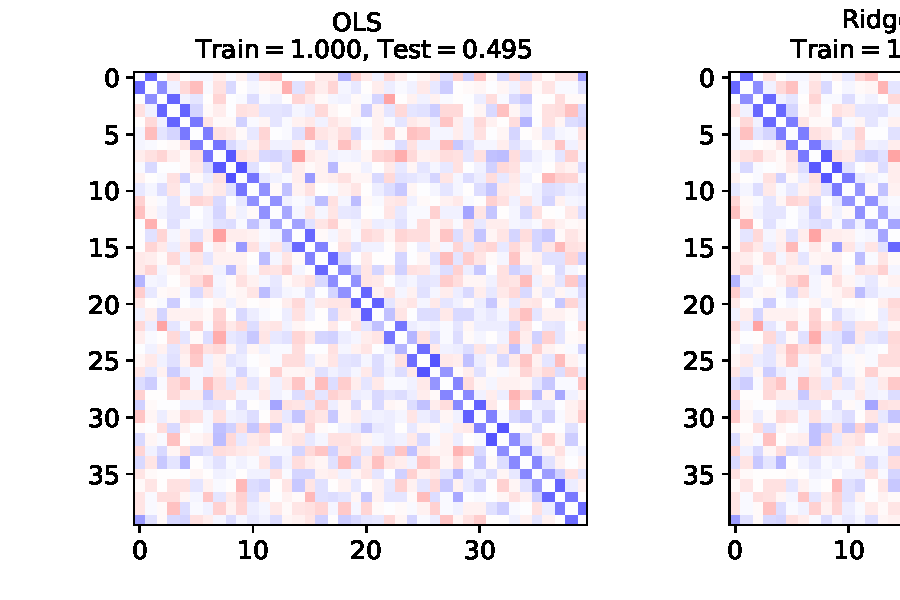
\includegraphics[scale=0.35]{latex/figures/ising_J_lmbda_10_0.pdf}}}
\qquad
\subfloat[]{{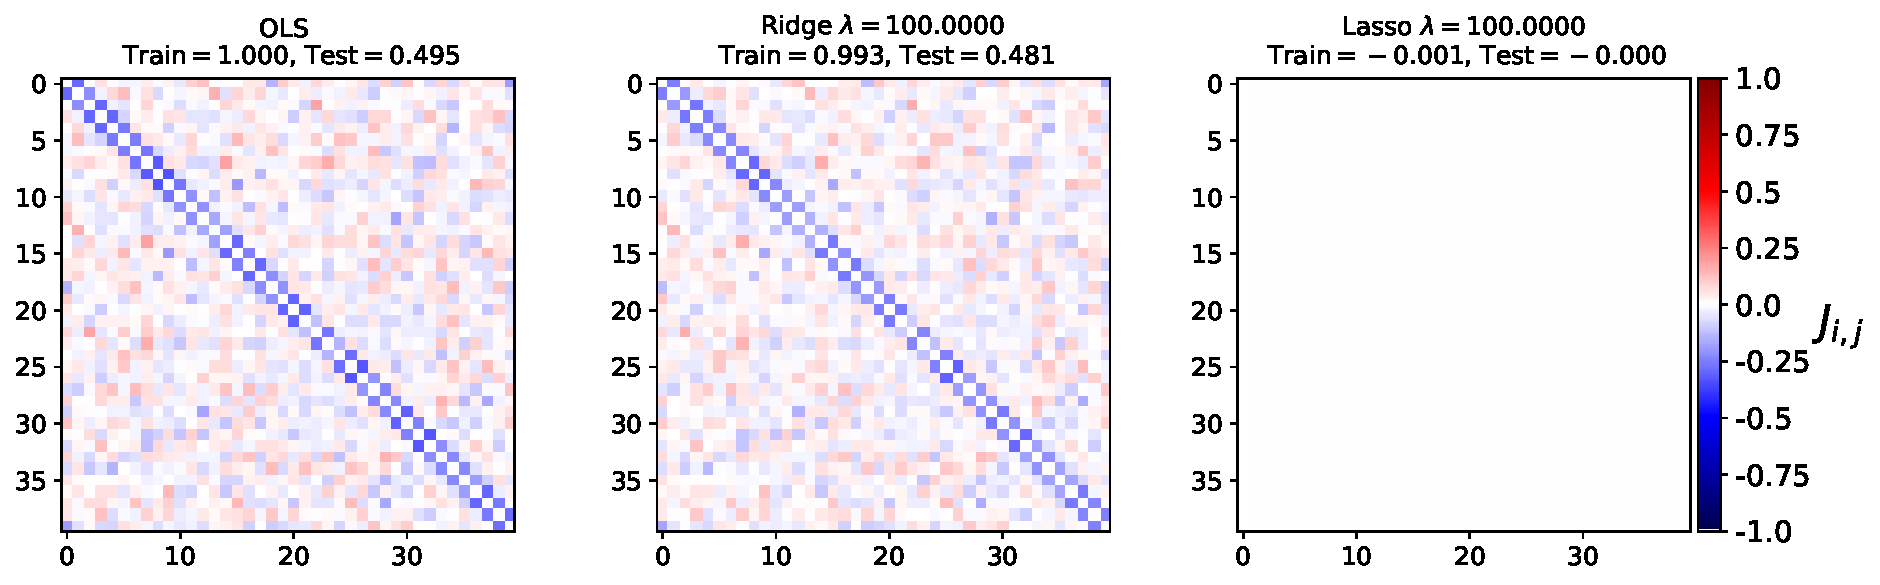
\includegraphics[scale=0.35]{latex/figures/ising_J_lmbda_100_0.pdf}}}
\qquad
\subfloat[]{{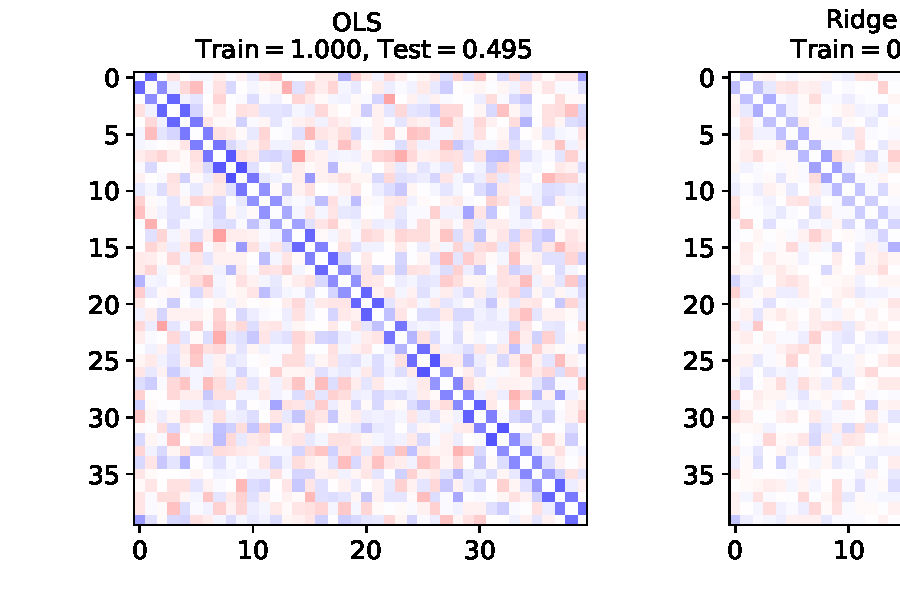
\includegraphics[scale=0.35]{latex/figures/ising_J_lmbda_1000_0.pdf}}}
\qquad
\subfloat[]{{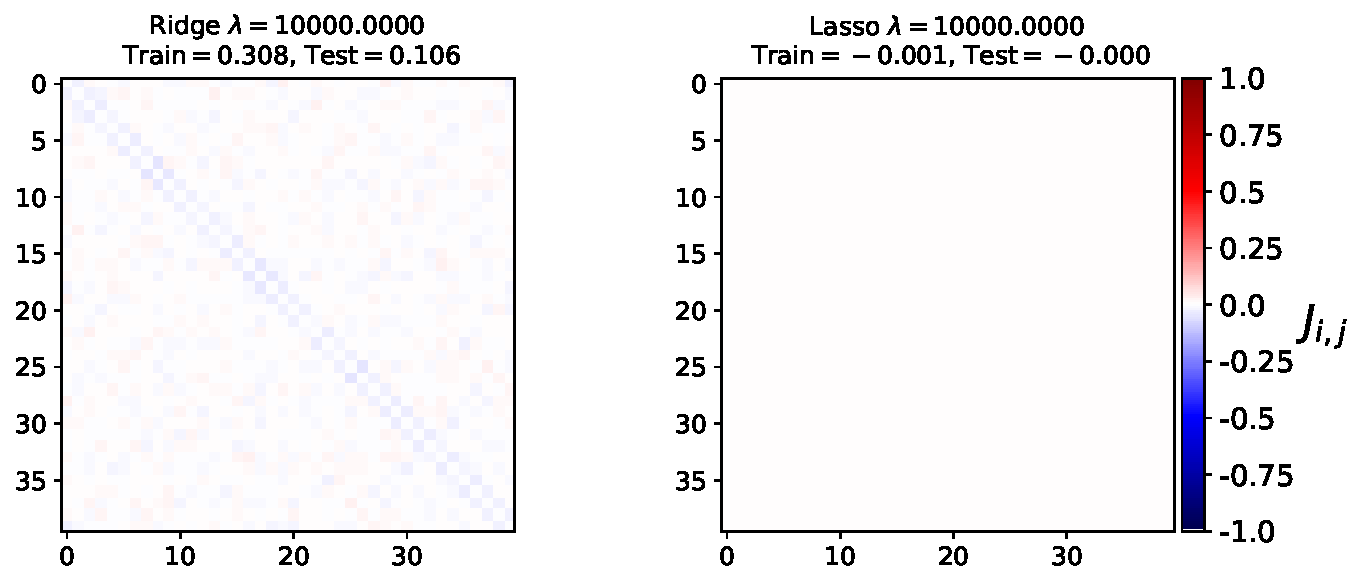
\includegraphics[scale=0.35]{latex/figures/ising_J_lmbda_10000_0.pdf}}}
\qquad
\subfloat[]{{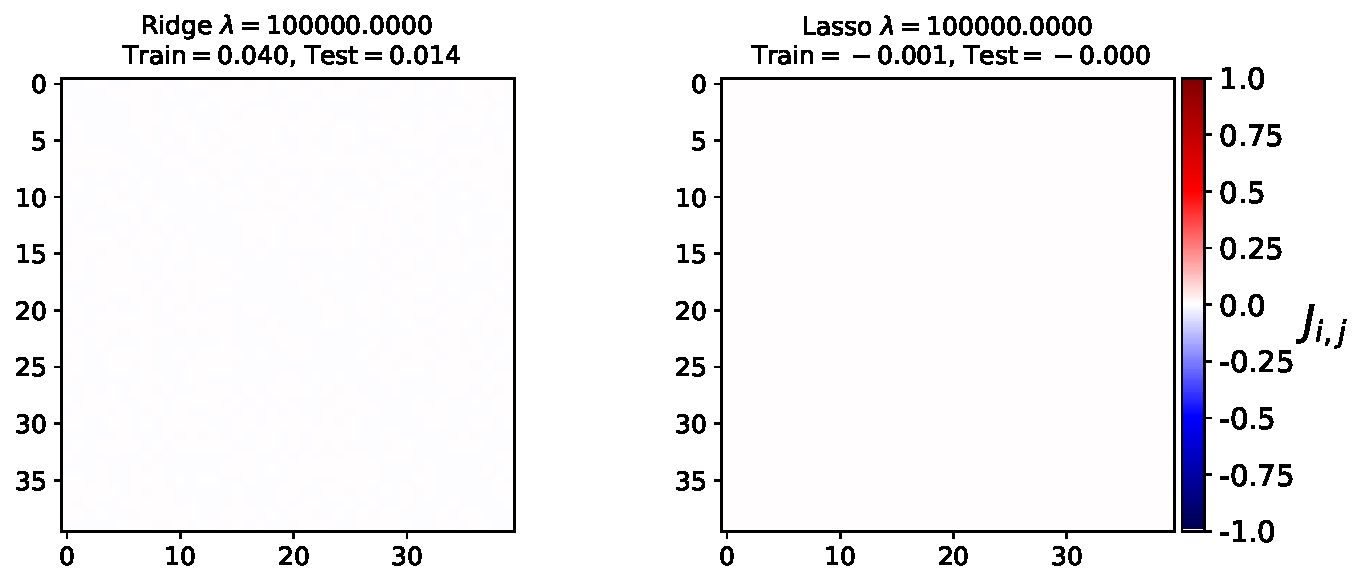
\includegraphics[scale=0.35]{latex/figures/ising_J_lmbda_100000_0.pdf}}}
\caption{figure text}
\label{fig:j_lmbda}
\end{figure}


\autoref{fig:performance_lmbda_1d} shows the $R^2$ score and MSE as a function of the regularization parameter $\lambda$.

\begin{figure}[H]
\centering
\subfloat[]{{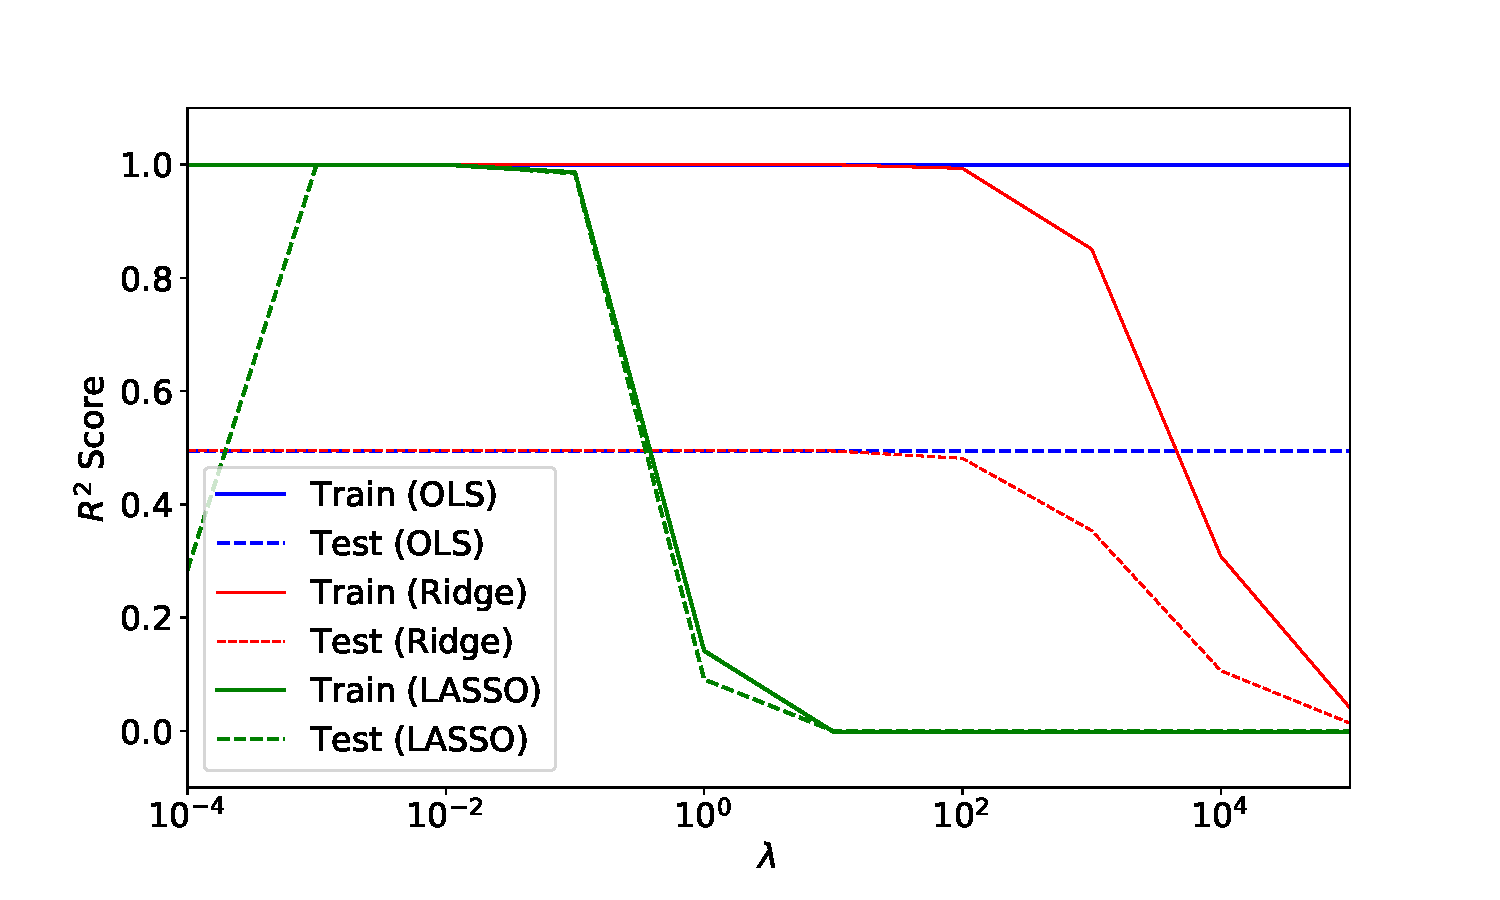
\includegraphics[scale=0.5]{latex/figures/ising1D_r2_vs_lmbda.pdf}}}
\qquad
\subfloat[]{{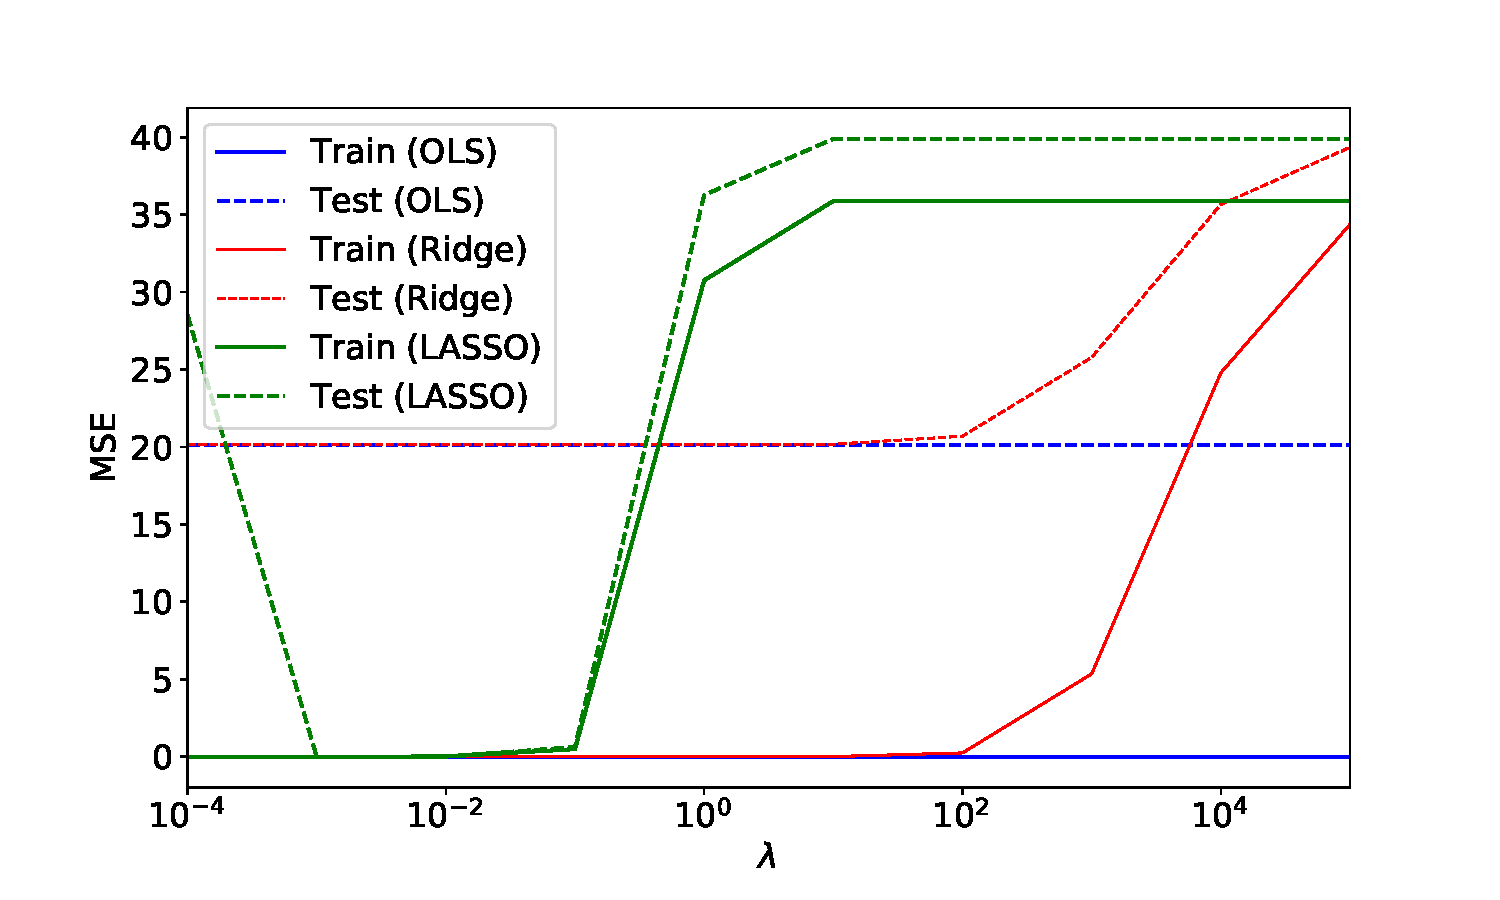
\includegraphics[scale=0.5]{latex/figures/ising1D_mse_vs_lmbda.pdf}}}
\caption{figure text}
\label{fig:performance_lmbda_1d}
\end{figure}


%----------------------------------------------------------------
\subsection{Identifying 2D Ising Model Phases with Logistic Regression}\label{sec:results logreg}
%----------------------------------------------------------------


%----------------------------------------------------------------
\subsection{Identifying 2D Ising Model Phases with Neural Networks}\label{sec:results NN}
%----------------------------------------------------------------